\documentclass[../main2.tex]{subfiles}
\begin{document}
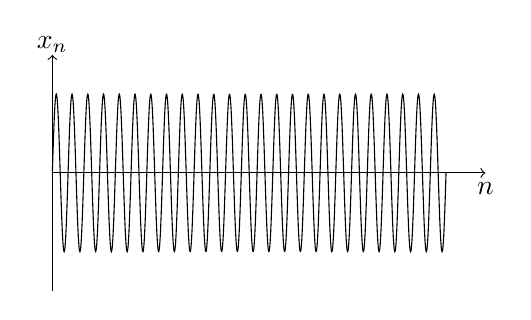
\begin{tikzpicture}[scale=1,baseline={(0,0)}]

%AXES
% horizontal axis
\draw[->] (0,0) -- (5.5,0) node[anchor=north] {$n$};
% vertical axis
\draw[->] (0,-1.5) -- (0,1.5) node[yshift=1em,anchor=north] {$x_n$};

%GRAPH
%input
%\draw[thick] (0,1.5) -- (1.8,1.5) -- (1.8,2.8) -- (3.5,2.8) -- (3.5,1.5) -- (5.5,1.5);
%output
%\draw[dashed,domain=0:3] plot (\x,{2+0.7*exp(-(\x)/0.25)});

%Input
\draw[samples=1000,domain=0:5] plot(\x,{sin(deg(2*pi*5*(\x)))});

%\draw[dashed] (3.5, 2) -- (3.5, 1);
%\draw[dashed,domain=3:5.5] plot (\x,{1.5-0.5*exp(-(\x-3)/0.3)});

%\draw(2.5, 3.3) node{{\scriptsize Attack phase}};
%\draw(4.5,0.6) node{{\scriptsize Release phase}};

\end{tikzpicture}
\end{document}
